\section{Diagramas de secuencia}\label{sec:diagramas}
\textbf{Importante}: en los siguientes diagramas optamos por aislar la clase \lstinline|App|, dado que se trata de una
clase puramente hecha para mostrar una posible ejecución.

\subsection{Agregar a wishlist}\label{subsec:agregar-a-wishlist}
\begin{figure}[h]
    \centering
    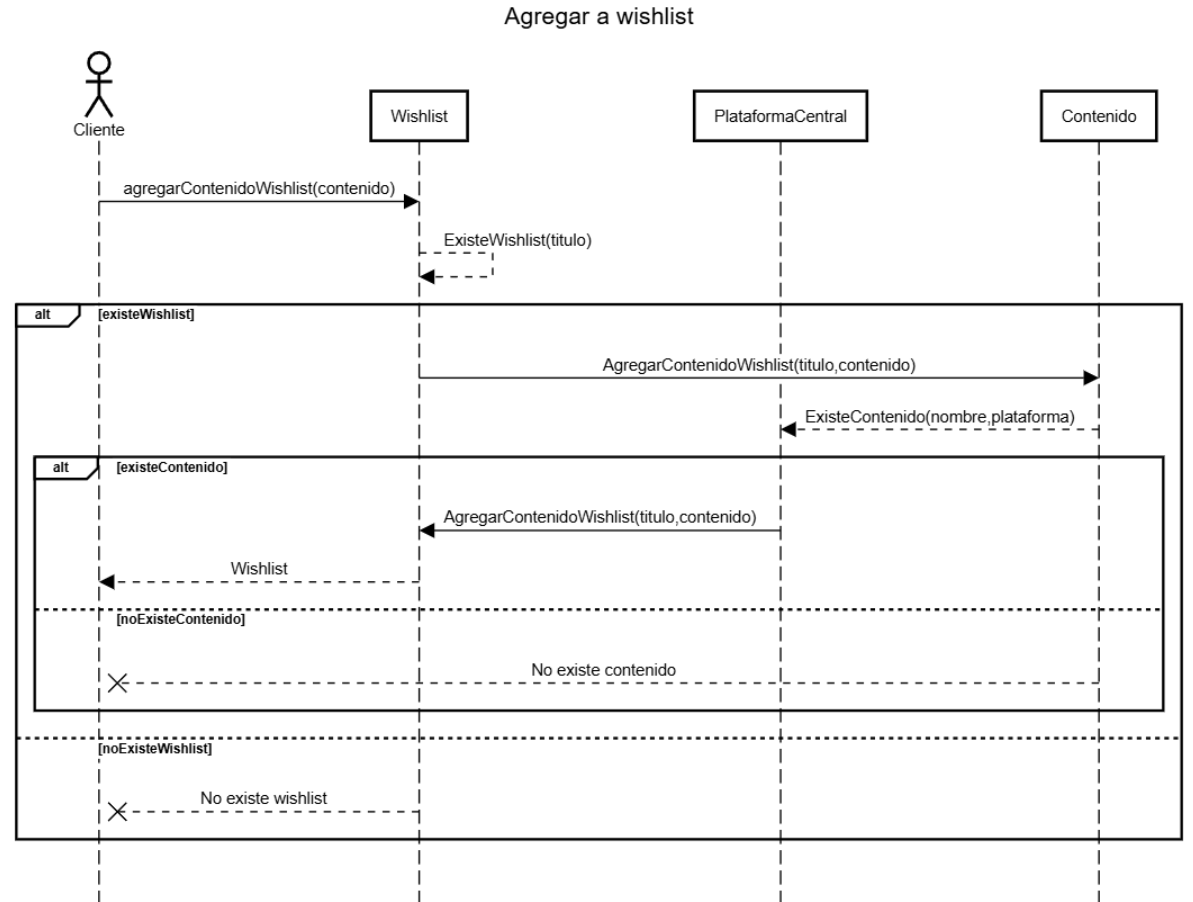
\includegraphics[width=1\textwidth]{img/agregar_a_wishlist.png}
\end{figure}

\clearpage

\subsection{Opinar y puntuar}\label{subsec:opinar-y-puntuar}
\begin{figure}[h]
    \centering
    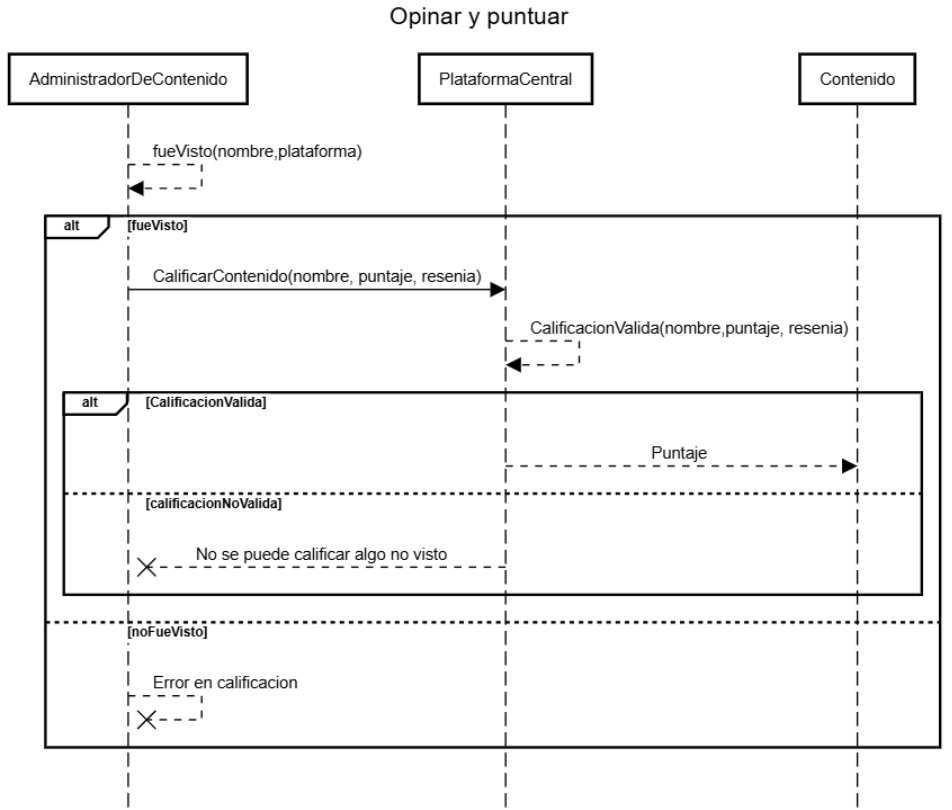
\includegraphics[width=0.8\textwidth]{img/opinar_y_puntuar.png}
\end{figure}

\subsection{Registrar cliente}\label{subsec:registrar-cliente}
\begin{figure}[h]
    \centering
    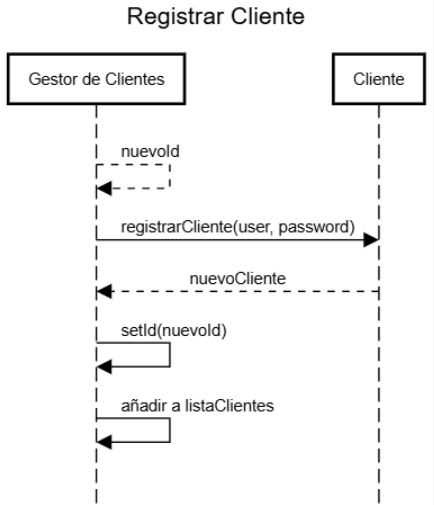
\includegraphics[width=0.4\textwidth]{img/registrar.png}
\end{figure}

\clearpage

\subsection{Últimos vistos}\label{subsec:ultimos-vistos}
\begin{figure}[h]
    \centering
    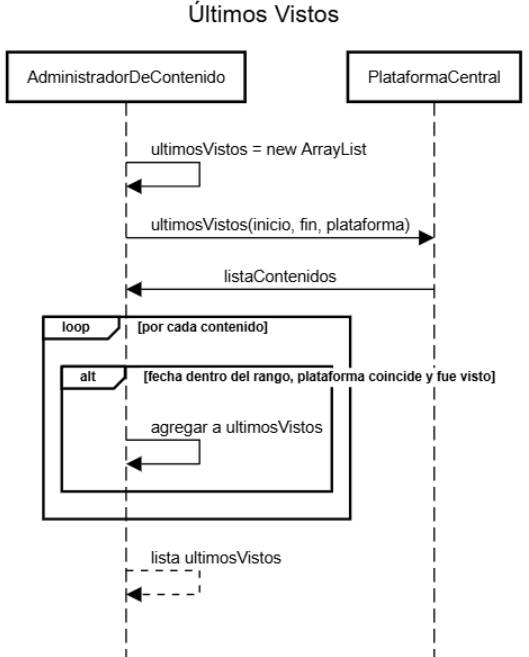
\includegraphics[width=0.9\textwidth]{img/ultimos_vistos.png}
\end{figure}

\clearpage

\subsection{Vistos}\label{subsec:vistos}
\begin{figure}[h]
    \centering
    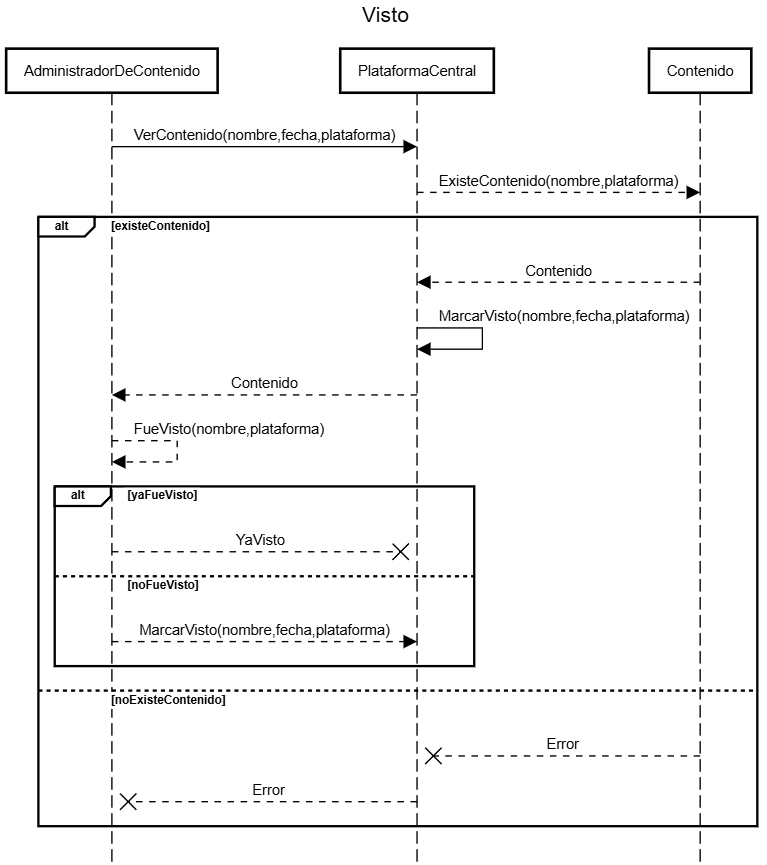
\includegraphics[width=1\textwidth]{img/visto.png}
\end{figure}

\clearpage

\section{Diagrama de clases}\label{sec:diagrama-de-clases}
\begin{figure}[h]
    \centering
    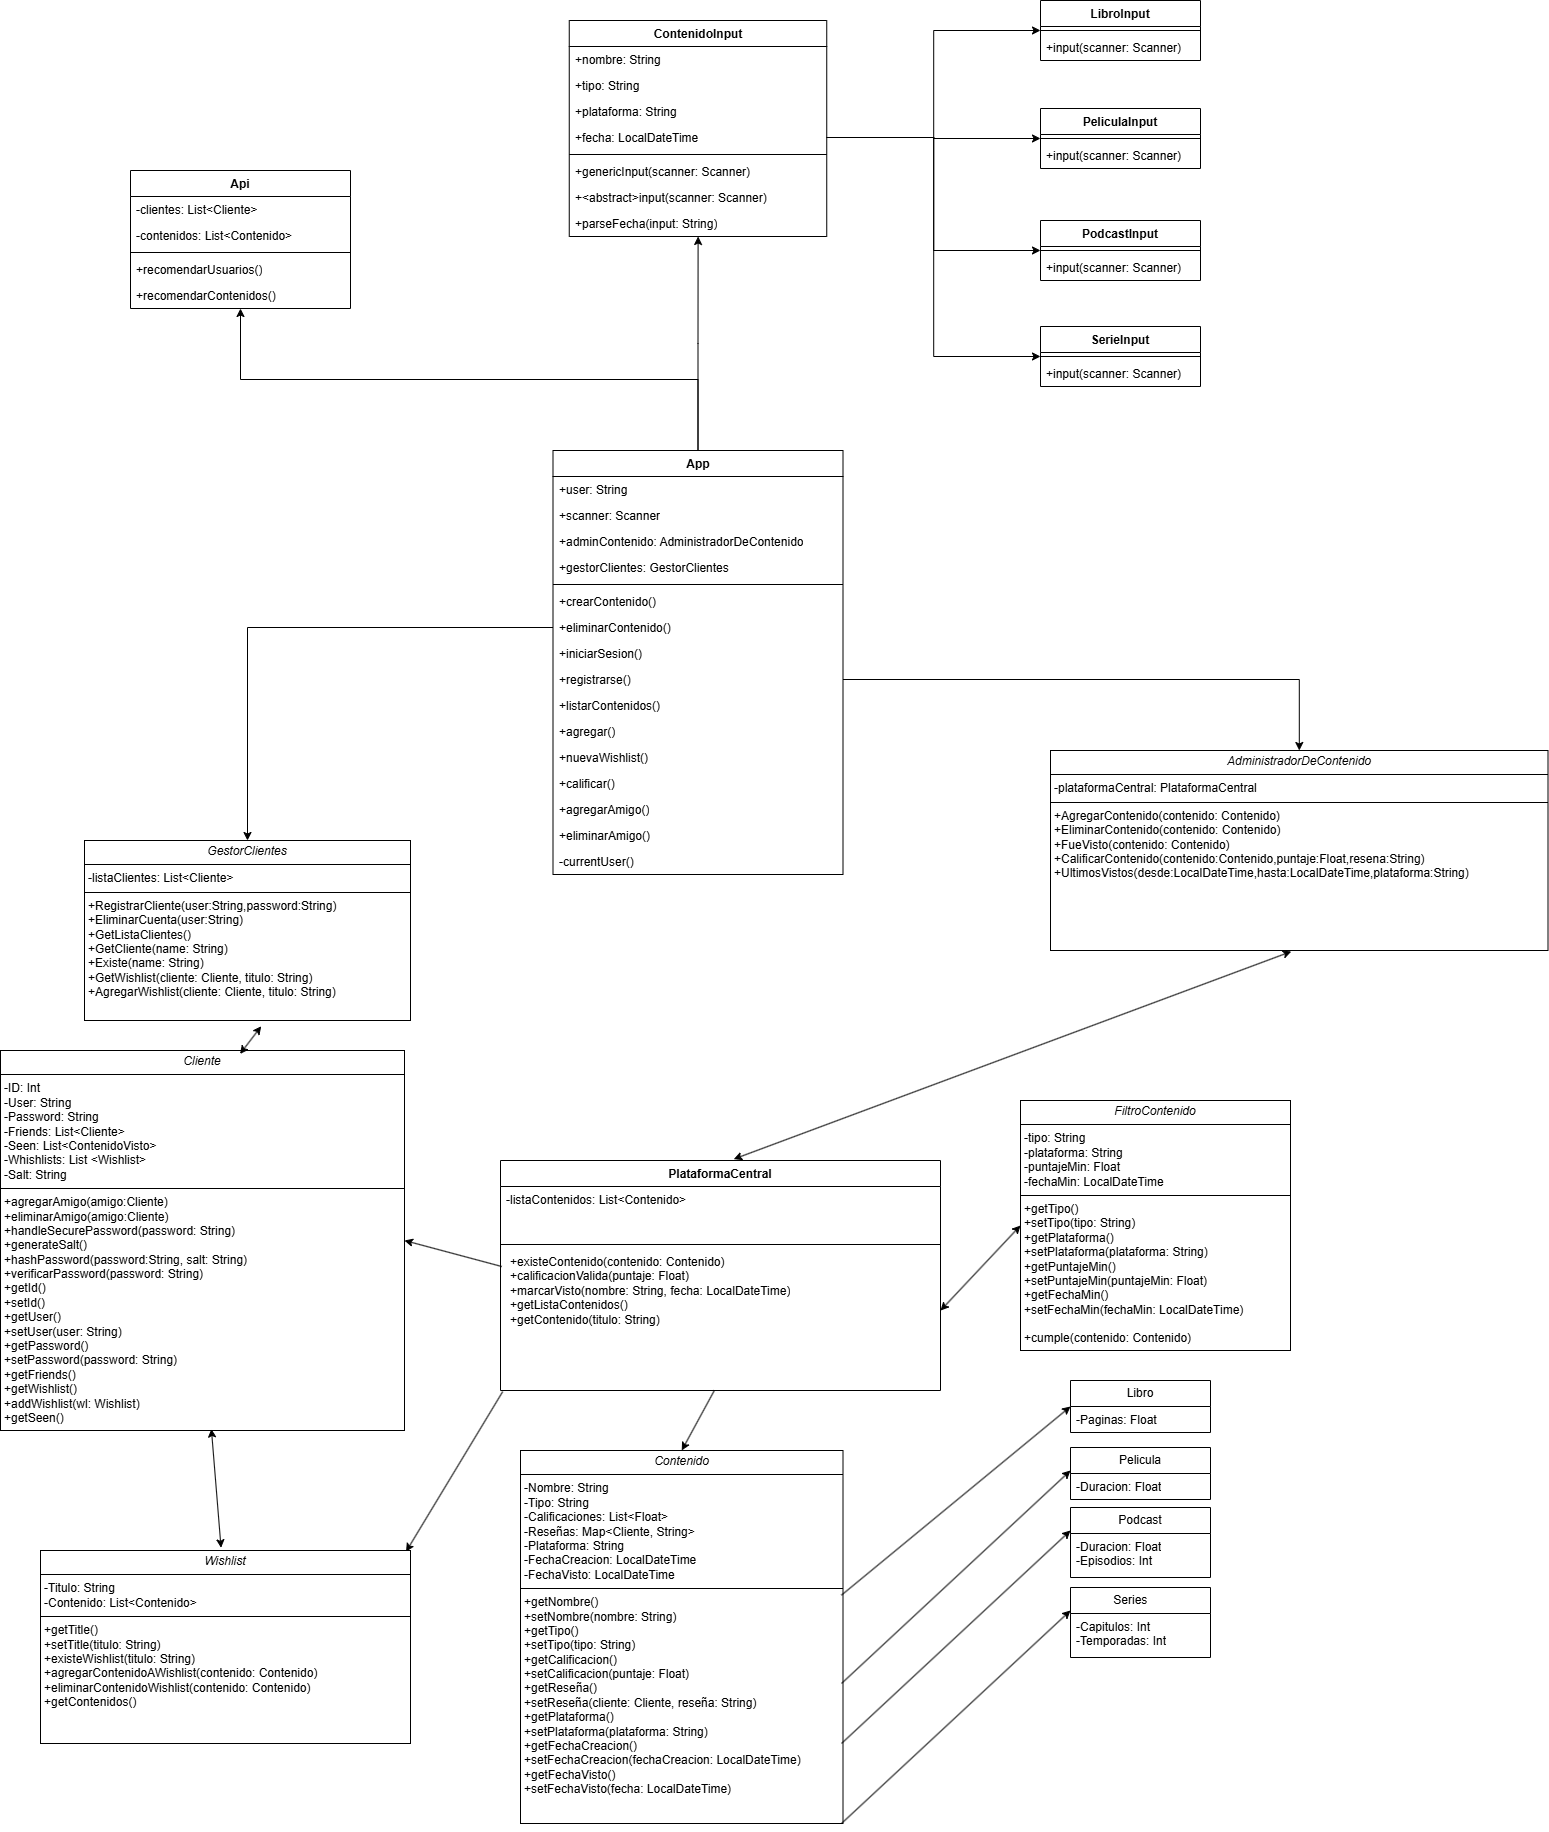
\includegraphics[width=1\textwidth]{img/diagrama_clases.png}
\end{figure}
